\begin{frame}
  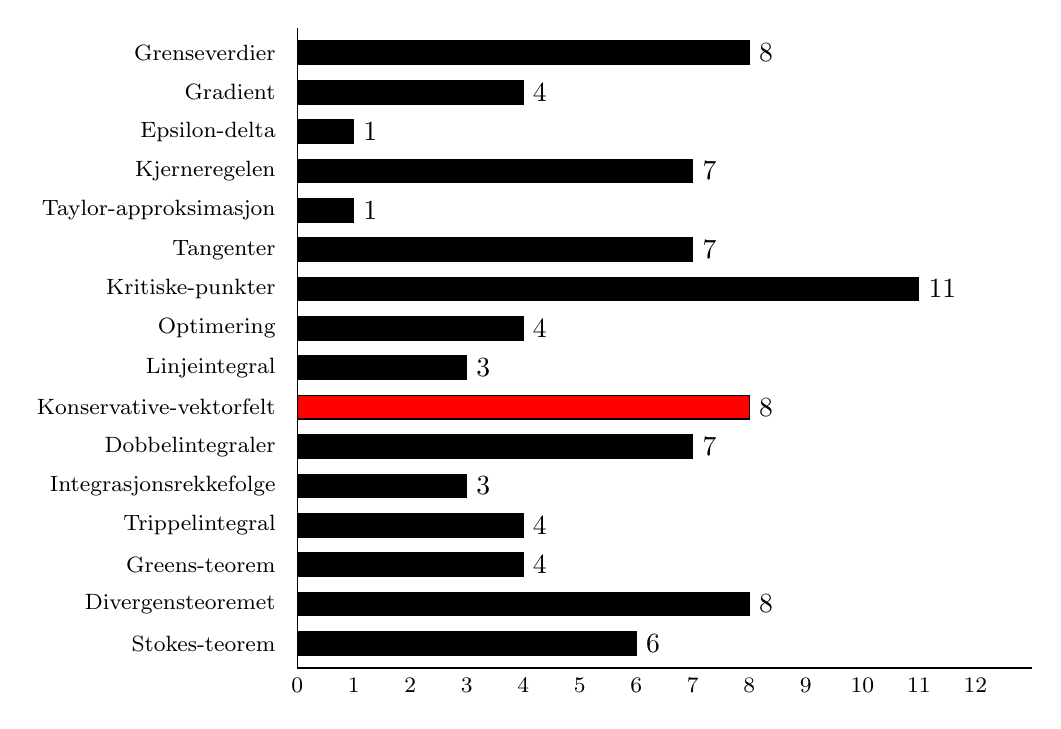
\begin{tikzpicture}
    \begin{axis}[ xbar=0pt, /pgf/bar shift=0pt, legend style={ legend columns=4,
        at={(xticklabel cs:0.5)}, anchor=north, draw=none }, ytick={0,...,15},
      ytick style={draw=none},% <- added
      axis y line*=none, axis x line*=bottom, tick label
      style={font=\footnotesize}, legend style={font=\footnotesize}, label
      style={font=\footnotesize}, xtick style={draw=none},% <- added
      xtick={0,1,...,12}, width=.9\textwidth, bar width=3mm, y dir = reverse,
      xmin=0, xmax=13, area legend,
      y=5mm, enlarge y limits={abs=0.625},
      style={text=black}, every axis plot/.append style={fill},
      nodes near coords, nodes near coords,
      yticklabels={%
        {\topicref{Grenseverdier}},
        {\topicref{Gradient}},
        {\topicref{Epsilon-delta}},
        {\topicref{Kjerneregelen}},
        {\topicref{Taylor-approksimasjon}},
        {\topicref{Tangenter}},
        {\topicref{Kritiske-punkter}},
        {\topicref{Optimering}},
        {\topicref{Linjeintegral}},
        {\topicref{Konservative-vektorfelt}},
        {\topicref{Dobbelintegraler}},
        {\topicref{Integrasjonsrekkefolge}},
        {\topicref{Trippelintegral}},
        {\topicref{Greens-teorem}},
        {\topicref{Divergensteoremet}},
        {\topicref{Stokes-teorem}}}]
      \addplot[fill=black] coordinates {(8,0)};
      \addplot[fill=black] coordinates {(4,1)};
      \addplot[fill=black] coordinates {(1,2)};
      \addplot[fill=black] coordinates {(7,3)};
      \addplot[fill=black] coordinates {(1,4)};
      \addplot[fill=black] coordinates {(7,5)};
      \addplot[fill=black] coordinates {(11,6)};
      \addplot[fill=black] coordinates {(4,7)};
      \addplot[fill=black] coordinates {(3,8)};
      \addplot[fill=red] coordinates {(8,9)};
      \addplot[fill=black] coordinates {(7,10)};
      \addplot[fill=black] coordinates {(3,11)};
      \addplot[fill=black] coordinates {(4,12)};
      \addplot[fill=black] coordinates {(4,13)};
      \addplot[fill=black] coordinates {(8,14)};
      \addplot[fill=black] coordinates {(6,15)};
    \end{axis}
  \end{tikzpicture}
\end{frame}

\begin{frame}
  \subsection{Konservative vektorfelt}\label{subsec:Konservative-vektorfelt}
  \frametitle{Konservative vektorfelt}
  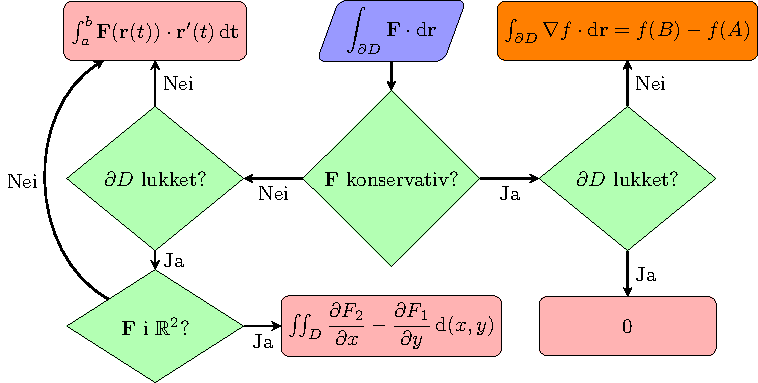
\includegraphics[scale=0.95]{../img/flytskjema-linjeintegral-2}
\end{frame}

\begin{frame}
  \frametitle{Konservative vektorfelt}
  \begin{definition}
    Et vektorfelt $\F \colon A \to \R^n$, hvor $A \subset \R^m$ er \emph{konservativt}
    dersom det eksisterer et skalarfelt $f$ med kontinuerlige partiellderiverte på
    $A$ slik at $\nabla f = (\frac{\partial f_1}{\partial x}, \frac{\partial
      f_2}{\partial y}) = (F_1, F_2) = \F$.
  \end{definition}
  \begin{theorem}
    \begin{itemize}
      \item $\F$ konservativt $\Longrightarrow$ $\curl \F = 0$
        \item Dersom følgende krav holder
        \begin{itemize}
          \item $\F$ er definert på et enkeltsammenhengende området $D$
          \item $\F$ har kontinuerlige partiellderiverte på hele $D$
          \item $\curl \F = 0$
        \end{itemize}
        Så har vi $\curl \F = 0$ $\Longrightarrow$ $\F$ konservativt.
    \end{itemize}
  \end{theorem}
\end{frame}

\begin{frame}
  \begin{oppgave}{V2015, Oppgave 8}
    La $\F \colon \R^3 \mapsto \R^3$ være gitt ved $\F(x, y, z) = yz\I +
    xz\J + xy\K$. Bestem
    % 
    \begin{equation*}
      \int_C \F \cdot \dr\,,
    \end{equation*}
    %
    når $C$ har parametriseringen $\rr(t) = (\cos t)\I + (\sin t)\J + t\K$, $0 \leq t < \pi/4$.
  \end{oppgave}
\only<1-4>{$\F$ er definert på hele $\R^3$ (enkeltsammenhengende) og har kontinuerlige partiellderiverte. Dersom
$\curl \F = \vek{0}$ så er $\F$ et konservativ felt.}%
\only<5>{Siden $\F$ er et konservativt felt eksisterer det et skalarfelt
  (potensial) $f$ slik at $\nabla f = (\frac{\partial f}{\partial x},
  \frac{\partial f}{\partial y}, \frac{\partial f}{\partial z}) = (yz, xz, xy) =
  \F$.}%
    \only<6->{Siden $f = xyz$, $\nabla f = \F$ og $\F$ er konservativt bruker vi
      formelen
      \begin{equation*}
        \only<6>{\int_C \nabla f \cdot \dr = f(B) - f(A)}
        \only<7->{\int_C \F \cdot \dr}
        \only<7>{ = f\bigl(\rr(\pi/4)\bigr) - f\bigl(\rr(0)\bigr)}
        \only<8>{ = f\bigl(\cos \tfrac{\pi}{4}, \sin \tfrac{\pi}{4}, \tfrac{\pi}{4}\bigr)
                  - f\bigl(\cos 0, \sin 0, 0\bigr)}
          \only<9>{= f(\tfrac{1}{\sqrt{2}}, \tfrac{1}{\sqrt{2}}, \tfrac{\pi}{4}) - f(1,0,0)}
          \only<10->{= \frac{\pi}{8}}
      \end{equation*} hvor $B$ og $A$ er
      henholdsvis start og sluttpunktet til kurven $C$.}
\only<2->{%
  \begin{align*}
    \only<2-4>{%
  \hspace{-0.2cm}
      \curl \F
    & = \nabla \times \F = 
  \begin{vmatrix}
    \I & \J & \K \\
    \frac{\partial}{\partial x} & \frac{\partial}{\partial y} & \frac{\partial}{\partial z}\\
    yz & xz & xy
  \end{vmatrix}}\only<3-4>{\\
    & = \I \left( \tfrac{\partial}{\partial y}(xy) - \tfrac{\partial}{\partial z}(xz) \right)
    - \J \left( \tfrac{\partial}{\partial x}(xy) - \tfrac{\partial}{\partial z}(yz) \right)
      + \K \left( \tfrac{\partial}{\partial x}(xz) - \tfrac{\partial}{\partial y}(yz) \right)\\}%
  \only<4>{
    & = \I \left( x - x \right)
    - \J \left( y - y \right)
      + \K \left( z - z\right)
      = \vek{0}}
  \only<5>{
      \diffp{f}{x} & = yz \Rightarrow f = xyz + C(y,z) \\
      \diffp{f}{y} & = xz \Rightarrow f = xyz + D(x,z) \\
      \diffp{f}{z} & = xy \Rightarrow f = xyz + E(x,y) 
    }
  \end{align*}}
\only<5>{Velger $C(y,z)=D(x,z)=E(x,y)=0$ slik at $f(x,y,z) = xyz$.}
\end{frame}

%%% Local Variables:
%%% mode: latex
%%% TeX-master: "main"
%%% End:
